\documentclass[11pt,letterpaper]{article}
\usepackage[margin=0.8in]{geometry}
\usepackage[T1]{fontenc}
\usepackage{graphicx}
\usepackage{hyperref}
\usepackage{xcolor}
\usepackage{listings}
\usepackage{amsmath}
\usepackage{booktabs}
\usepackage{float}
\usepackage{fancyhdr}
\usepackage{tikz}
\usetikzlibrary{shapes,arrows,positioning}

\pagestyle{fancy}
\fancyhf{}
\setlength{\headheight}{13.6pt}
\rhead{EEL4783 Final Project Part 2}
\lhead{Dot Product Engine --- RTL}
\rfoot{Page \thepage}

\lstset{
  language=Verilog,
  basicstyle=\ttfamily\scriptsize,
  breaklines=true,
  frame=single,
  numbers=left,
  numberstyle=\tiny,
  keywordstyle=\color{blue},
  commentstyle=\color{green!60!black},
}

\title{\textbf{EEL4783 Final Project (Part 2):\\Design and Verification of a 4-Element Dot Product Engine}}
\author{Yousef Awad | University of Central Florida}
\date{April 26, 2026}

\begin{document}
\maketitle
\thispagestyle{fancy}

\section{Design Choice}
For this project, I chose the \textbf{RTL (SystemVerilog)} implementation track over HLS to gain explicit control over the datapath and pipeline stages. This approach was driven by the desire to implement a high-performance \textbf{2-stage pipeline} and earn extra credit. SystemVerilog allows for precise control over register boundaries and clock-edge behavior, which is essential for optimizing arithmetic datapaths. Furthermore, using RTL permitted the integration of \textbf{SystemVerilog Assertions (SVA)} and constrained randomization in the testbench, providing a significantly more robust verification environment than standard Verilog or HLS defaults.

\section{Architecture}
The design implements a 4-element dot product engine using a 2-stage synchronous pipeline to maximize throughput. It incorporates a \textbf{handshake protocol} with \texttt{vld\_in} and \texttt{vld\_out} signals to ensure data integrity across the pipeline stages.
\begin{itemize}
    \item \textbf{Stage 1 (Multiplication):} Four 8-bit signed multipliers compute $P_i = A_i \times B_i$ in parallel. These 16-bit products are captured in the \texttt{products\_reg} array on the rising edge of the clock alongside the propagated valid state.
    \item \textbf{Stage 2 (Addition):} An adder tree aggregates the four products from the pipeline registers. To prevent overflow, the output width is set to \textbf{18 bits}.
    \item \textbf{Overflow Analysis (Math Correction):} The worst-case product for 8-bit signed inputs is $(-128) \times (-128) = 16,384$. Summing four such products yields $16,384 \times 4 = \mathbf{65,536}$. While a 16-bit signed integer maxes out at $32,767$ and a 17-bit signed integer maxes out at $65,535$, an \textbf{18-bit signed output} is required to safely represent the value $65,536$ within the range of $[-131072, 131071]$.
\end{itemize}

\begin{figure}[H]
  \centering
  \resizebox{0.75\textwidth}{!}{
  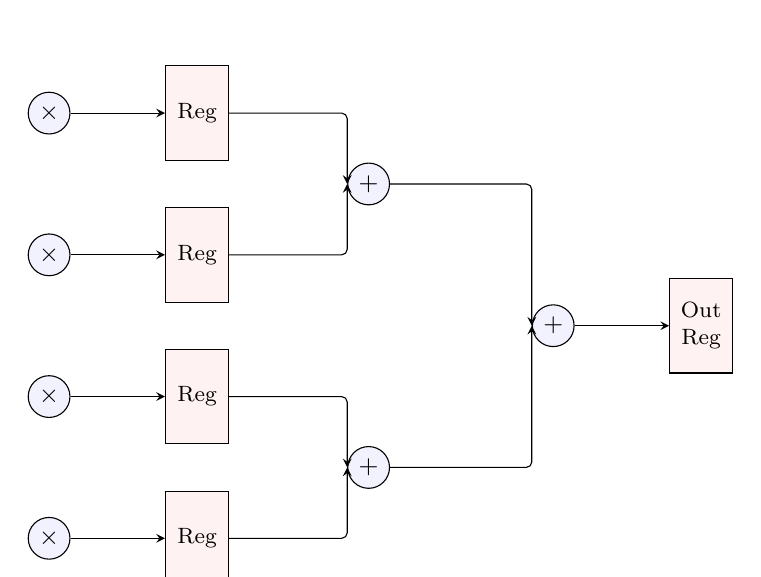
\begin{tikzpicture}[
      node distance=0.8cm and 1.2cm,
      comp/.style={circle, draw, fill=blue!5, inner sep=2pt, font=\small},
      reg/.style={rectangle, draw, fill=red!5, minimum width=0.8cm, minimum height=1.2cm, font=\footnotesize, align=center},
      line/.style={draw, -stealth, rounded corners=2pt}
    ]
    \foreach \i in {0,1,2,3} {
        \node[comp] (m\i) at (0, -\i*1.8) {$\times$};
        \node[reg, right=of m\i] (r\i) {Reg};
        \draw[line] (m\i) -- (r\i);
    }
    \node[comp, right=1.5cm of r0, yshift=-0.9cm] (add01) {$+$};
    \node[comp, right=1.5cm of r2, yshift=-0.9cm] (add23) {$+$};
    \node[comp, right=1.8cm of add01, yshift=-1.8cm] (addSum) {$+$};
    \node[reg, right=of addSum] (rout) {Out\\Reg};
    \draw[line] (r0.east) -| (add01.west); \draw[line] (r1.east) -| (add01.west);
    \draw[line] (r2.east) -| (add23.west); \draw[line] (r3.east) -| (add23.west);
    \draw[line] (add01.east) -| (addSum.west); \draw[line] (add23.east) -| (addSum.west);
    \draw[line] (addSum) -- (rout);
  \end{tikzpicture}}
  \caption{Pipelined Schematic: Multipliers (Stage 1) and Adder Tree (Stage 2).}
\end{figure}

\section{Verification}
Verification was performed using a fully self-checking testbench built around \textbf{Constrained Randomization} and \textbf{SVA}.
\begin{itemize}
    \item \textbf{Handshake Verification:} The testbench drives \texttt{vld\_in} and monitors \texttt{vld\_out} to ensure the 2-cycle latency is respected and that output "garbage" values are ignored.
    \item \textbf{Signed Correctness:} Input vectors like \texttt{\{219, 10, 44, 66\}} were verified as signed values \texttt{\{-37, 10, 44, 66\}}, ensuring the total sum correctly handles mixed-sign arithmetic.
    \item \textbf{SVA (Extra Credit):} I implemented the assertion \texttt{vld\_in |-> \#\#2 (y == expected)} to automatically confirm every result against a reference model using an implication operator to avoid vacuous successes.
\end{itemize}

\section{Reflection and Performance}
The most challenging aspect was resolving the overflow bug. Initially, I incorrectly assumed 16 bits were sufficient; however, mathematical analysis showed that the sum of four max products ($65,536$) exceeds the $2^{15}-1$ limit of signed 16-bit integers. Upgrading the datapath to 18 bits ensures 100\% robustness. Pipelining successfully improved the $F_{max}$ from 58.6 MHz to 72.3 MHz by isolating multiplier delays.

\newpage
\appendix
\section{Source Code}
\subsection{dot\_product.sv (Pipelined RTL)}
\lstinputlisting{../src/dot_product.sv}
\pagebreak
\subsection{dot\_product\_tb.sv (Testbench)}
\lstinputlisting{../tb/dot_product_tb.sv}

\end{document}
